\chapter{Implementation}
\label{implementation}

% summary
In this chapter, the tools and techniques used in building this \gls{vr}-based \gls{hri} system are described. Particular emphasis is given to the interaction techniques for different operation modes. In addition, the setup of the robot and the construction of test scenes will also be covered in this chapter.


\section{Overview}
One of the aims of this thesis is to design and implement a \gls{vr}-based \gls{hri} system with different methods of operating the robot in order to find out which operation method is more suitable to control the rescue robot. Further, this thesis aims to provide some fundamental insights for future development directions and to provide a general direction for finding an intuitive, easy-to-use and efficient interaction approach for \gls{hri}. Therefore, the proposed system was developed using \gls{unity}, including four operation modes and corresponding test scenes for simulating post-disaster scenarios. In each operation mode, the user has a different method to control the robot. In addition, the system should simulate the process by which the robot scans its surroundings and the computer side cumulatively gets a reconstructed 3D virtual scene. The test environment was thus implemented in such a way that the scene seen by the user depends on the robot's movement and the trajectory it travels through.

\section{System Architecture}
% The proposed system runs on a computer with the Windows 10 operating system. This computer has been equipped with an Intel Core i7-8700K CPU, 32 GB RAM as well as a NVIDIA GTX 1080 GPU with 8 GB VRAM. \gls{htc} is used as a \gls{vr} device. It has a resolution of 1080 × 1200 per eye, resulting in a total resolution of 2160 × 1200 pixels, a refresh rate of 90 Hz, and a field of view of 110 degrees. It includes two motion controllers and uses two Lighthouses to track the headset's position and the motion controllers.
The proposed system uses \gls{htc} as \gls{vr} device. It has a resolution of 1080 × 1200 per eye, resulting in a total resolution of 2160 × 1200 pixels, a refresh rate of 90 Hz, and a field of view of 110 degrees. It includes two motion controllers and uses two Lighthouses to help track the headset's position and the motion controllers.

\gls{unity} was chosen as the platform to develop the system. \gls{unity} is a widely used game engine with \gls{steamvr} \footnote{https://assetstore.unity.com/packages/tools/integration/steamvr-plugin-32647}, which allows developers to focus on the \gls{vr} environment and interactive behaviors in programming, rather than specific controller buttons and headset positioning, making \gls{vr} development much simpler. Another reason why \gls{unity} was chosen as a development platform was its potential for collaboration with \gls{ros}, a frequently used operating system for robot simulation and manipulation, which is flexible, low-coupling, distributed, open source, and has a powerful and rich third-party feature set. In terms of collaboration between \gls{unity} and \gls{ros}, Siemens provides open-source software libraries and tools in C\# for communicating with ROS from .NET applications \footnote{https://github.com/siemens/ros-sharp}. Combining \gls{ros} and \gls{unity} to develop a collaborative \gls{hri} platform proved to be feasible \cite{Whitney:2018wk}. Since the focus of this work is on \gls{hri}, collaboration and synchronization of \gls{ros} will not be explored in detail here.

\section{Robot}
The proposed system needs to simulate the process that a robot uses a \gls{lidar} remote sensor to detect the real environment and synchronize it to \gls{unity}. Thus, a sphere collision body was set up on the robot as seen in \ref{fig:robot}. The collider is an invisible \gls{unity} component that can interact with other colliders by collision detection and a trigger event (onTriggerEnter function). In this system, the sphere collision body defines the range of the robot's \gls{lidar} detection. It will interact with invisible objects in the scene, such as buildings, during the robot's movement, and transform the Layers of the objects into visible Layers. The robot's driving performance, such as the number of collisions, average speed, total distance, will be recorded in each test. The detailed recorded information can be seen in Chapter \ref{result}. The movement of the robot depends on the value of the signal that is updated in each mode. In addition, the robot's Gameobject has the \gls{nav} \footnote{https://docs.unity3d.com/ScriptReference/AI.NavMeshAgent.html} component, which supports the robot's navigation to the specified destination with automatic obstacle avoidance in the test scene. The virtual robot has three cameras. One of the cameras is a simulation of a surveillance camera mounted on the robot, which can see all the items in the scene, although the distant items are not yet detected by LiDAR. Two of these cameras are set up in such a way that they can only see the area detected by \gls{lidar}. Each camera captures what it sees and modifies the bound image in real time. The four operation modes described later all use the camera viewport as a monitoring screen by rendering the camera viewport on UI canvas.


\begin{figure}[htbp]
    \centering
    \subfigure[LiDAR Collider]{
        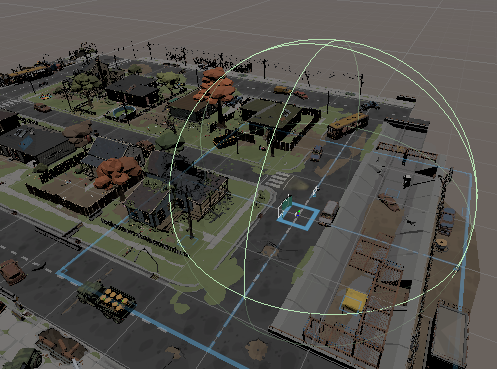
\includegraphics[height=5cm]{graphics/robot2.png}
    }
    \subfigure[Surveillance camera]{ 
        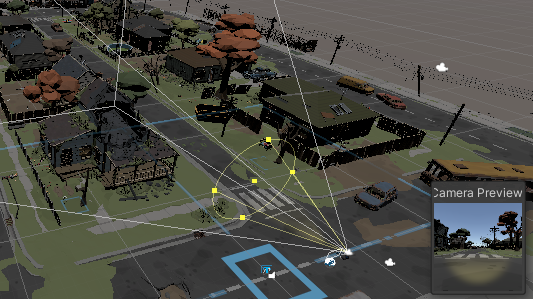
\includegraphics[height=5cm]{graphics/robot4.png}
    }
    \caption{Robot}
    \label{fig:robot} 
\end{figure}



\section{Interaction techniques}
This system has four different approaches to control the robot. Each mode has its own distinctive features: 

\begin{enumerate}
\item In Handle Mode, the user will send control commands directly using the motion controller. 
\item In Lab Mode, a simulated lab is constructed in the \gls{vr} environment and the user will use virtual buttons in the lab to control the rescue robot. 
\item In Remote Mode, the user can set the driving destination directly. 
\item In UI Mode, the user has a virtual menu and sends commands via rays from the motion controller.
\end{enumerate}

In order to improve the reusability of the code and facilitate the management of subsequent development, the classes that manage the interaction actions of each mode implement the same interface. A graphical representation of the system structure is given in the UML activity diagram in Figure \ref{fig:uml}.

\begin{figure}[htbp]
    \centering
    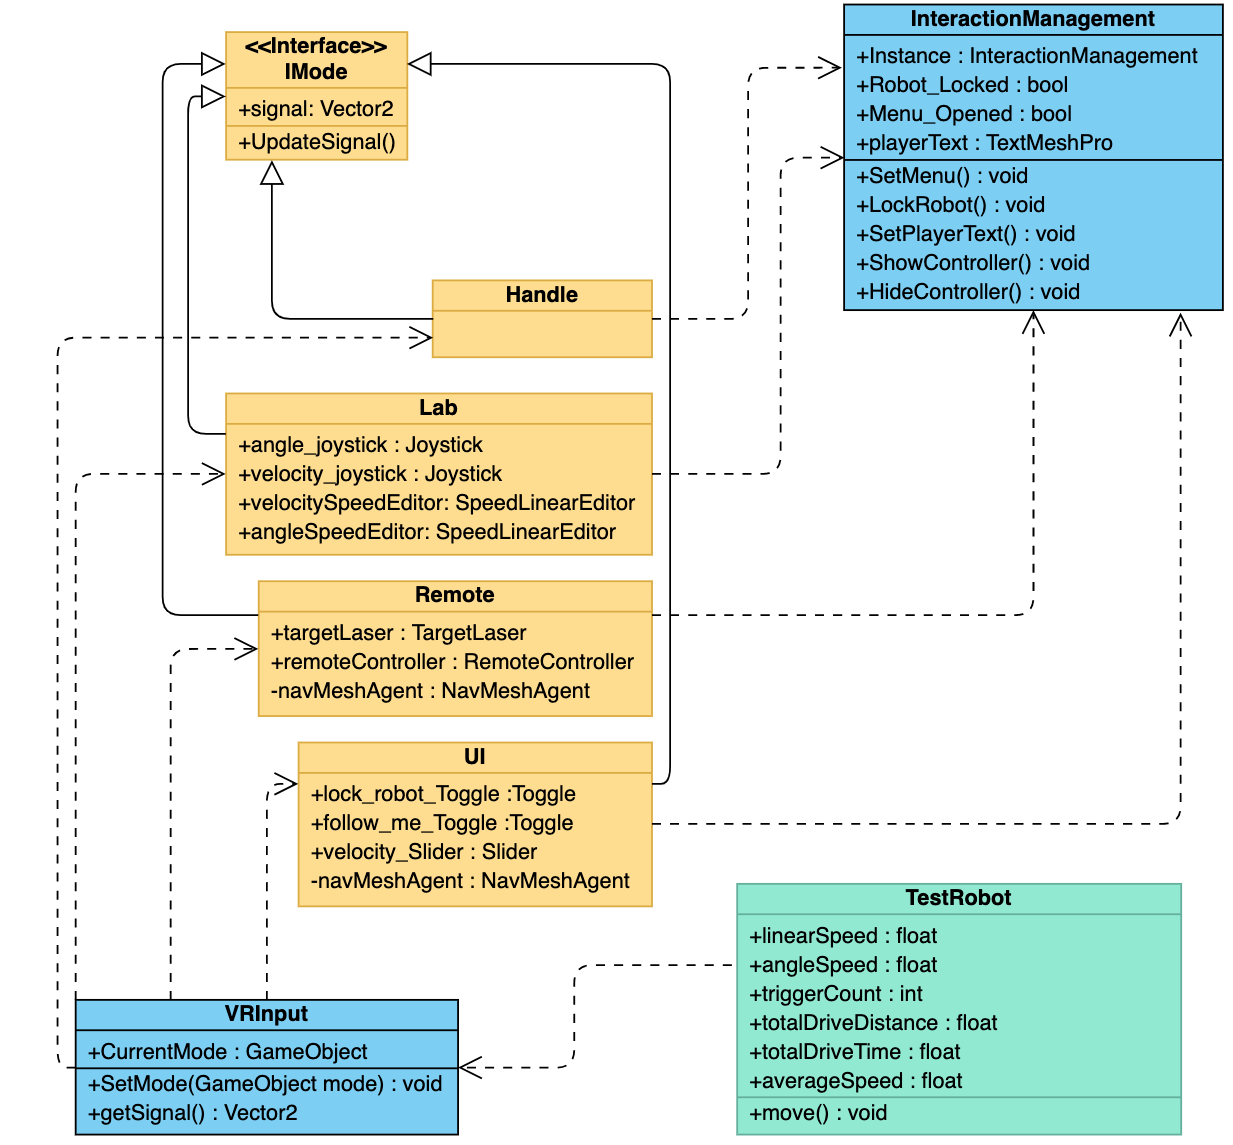
\includegraphics[width=\textwidth]{graphics/uml.png}
    \caption{UML Class diagram for the main structure of the system}
    \label{fig:uml}
\end{figure}

\subsection{Handle Mode}
In this mode, the user controls the robot's movement directly through the motion controller in the right hand. The touchpad of the motion controller determines the direction of rotation of the robot. The user can control the robot's driving speed by pulling the Trigger button. Figure \ref{fig:htc} shows the \gls{htc} motion controller. The robot rotation direction will read the value of the touchpad X-axis. The range of values is $[-1,1]$. Forward speed reads the Trigger button passed in as a variable of type SteamVR\_Action\_Single, and the range of the variable is $[0,1]$. With the right-hand menu button, the surveillance screen can be turned on or off. The monitor window can be adjusted to a suitable position by dragging and rotating it. In the literature dealing with \gls{vr} and \gls{hri}, many researchers have used a similar operational approach. Therefore, as a widely used, and in a sense default operation approach, this mode was designed as one of the operation modes.

\begin{figure}[htbp]
    \centering
    \begin{minipage}[t]{0.48\textwidth}
        \centering
        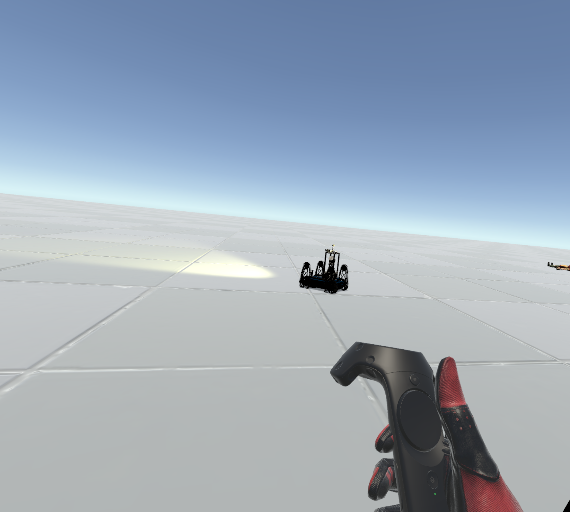
\includegraphics[height=5cm]{graphics/handle1.png}
        \caption{Handle Mode}
        \label{fig:handle}
    \end{minipage}
    \begin{minipage}[t]{0.48\textwidth}
        \centering
        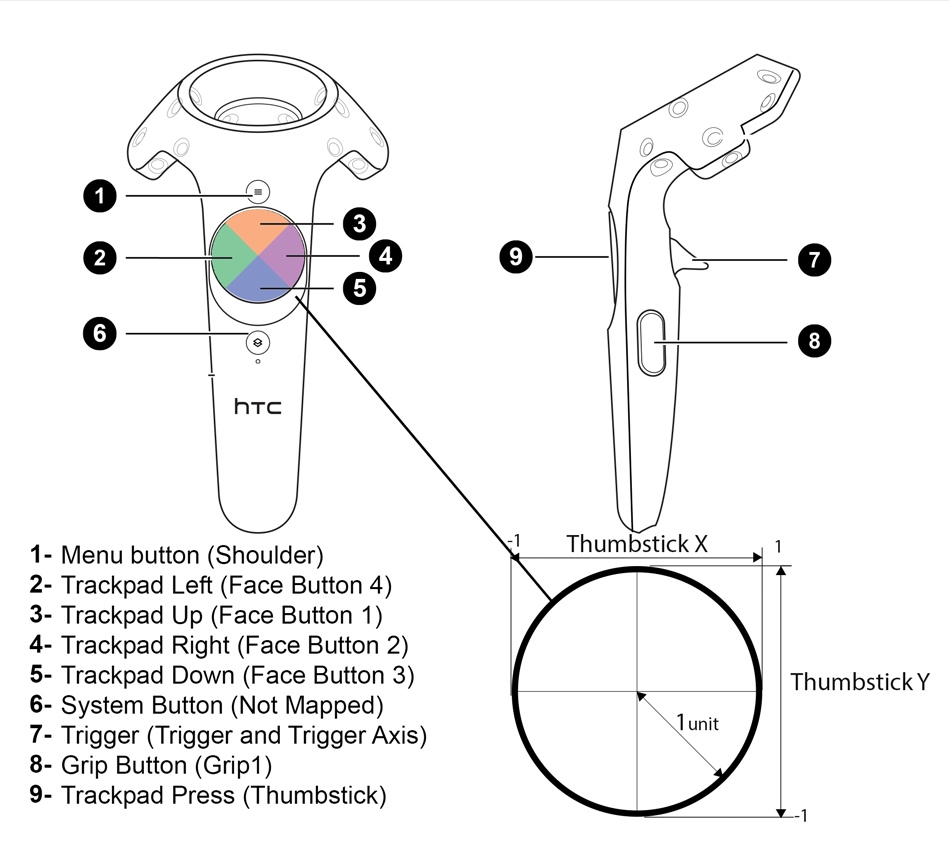
\includegraphics[height=5cm]{graphics/htc.png}
        \caption{HTC handle illustration}
        \label{fig:htc}
    \end{minipage}
\end{figure}


\subsection{Lab Mode}
This pattern was designed with reference to the system proposed by \cite{Matsas:2017aa}\cite{Perez:2019ub}. Their frameworks are used to train operators to work with the robot, avoiding risks and saving learning costs. In addition, they also mentioned that being in a simulated factory or laboratory can improve immersion. Therefore, in this mode, a virtual laboratory environment is constructed, in which simulated buttons, controllers, and monitoring equipment are placed. The laboratory consists of two parts. The first part is the monitoring equipment: the monitoring screen is enlarged and placed at the front of the lab as a huge display. The second part is the operating console in the center of the laboratory, which can be moved by the user as desired. This is due to the fact that users have different heights and may wish to operate the robot in a standing or sitting position. The user can use the buttons on the table to lock the robot or let it move forward automatically. In the middle of the console are two operating joysticks that determine the robot's forward motion and rotation respectively. The part that involves virtual joystick movement and button effects uses an open-source GitHub project VRtwix\footnote{https://github.com/rav3dev/vrtwix}. With the sliding stick on the left, the user can edit the speed of the robot's forward movement and rotation.

\begin{figure}[htbp]
    \centering
    \subfigure[Overview]{
        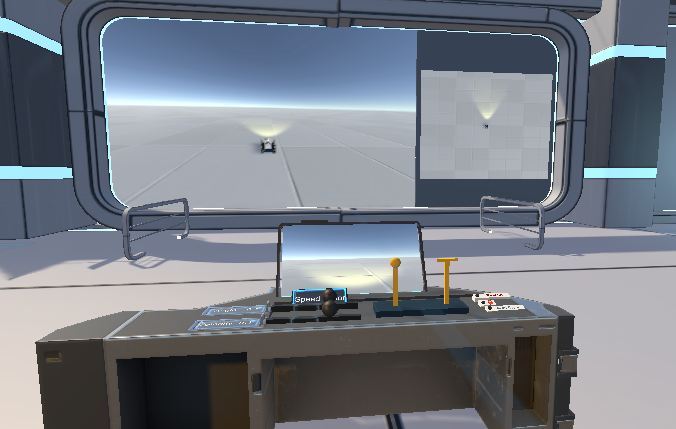
\includegraphics[height=5cm]{graphics/lab1.png}
    }
    \subfigure[Operating console]{ 
        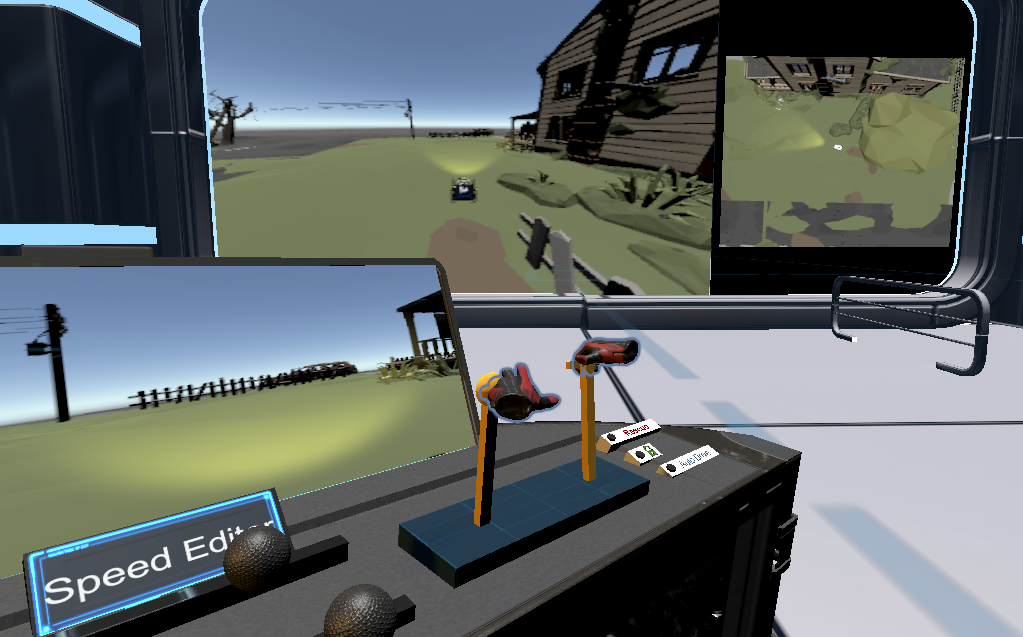
\includegraphics[height=5cm]{graphics/lab3.png}
    }
    \caption{Lab Mode}
    \label{fig:lab} 
\end{figure}

\subsection{Remote Mode}
In this mode, the user can set the driving target point directly or control the robot by picking up the remote control placed on the toolbar. The target point is set by the ray emitted by the right motion controller. This process is similar to setting a teleportation point. After the target point is set, a square representing the destination is shown in the scene, and the robot will automatically travel to the set destination. The entire driving process uses the \gls{nav} component and is therefore capable of automatic obstacle avoidance.
A movable toolbar with remote control and a monitoring device can be opened by clicking on the menu button. The remote control is a backup precaution if the automatic navigation fails to navigate the target point properly. The user can adjust the direction of the robot's travel by using the remote control. The pickup and auto-release parts use the ItemPackage component available in the \gls{steamvr}.

\begin{figure}[htbp]
    \centering
    \subfigure[Overview]{
        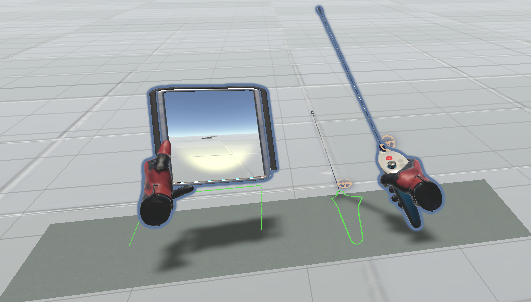
\includegraphics[height=5cm]{graphics/remote2.png}
    }
    \subfigure[Set the destination]{ 
        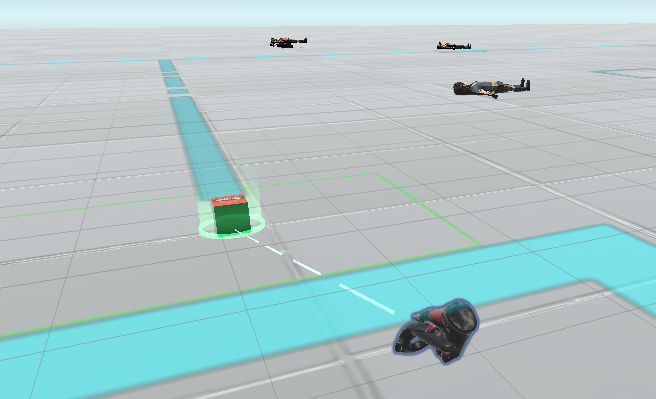
\includegraphics[height=5cm]{graphics/remote3.png}
    }
    \caption{Remote Mode}
    \label{fig:remote} 
\end{figure}


\subsection{UI Mode}
The virtual menu is also an interaction method that is often used in \gls{vr}, so this mode is proposed. In this mode, the user interacts with the virtual menu using the ray emitted by the right motion controller. The virtual menu is set up with buttons for the direction of movement, a speed controller, and buttons to open and close the monitor screen. In addition to this, an additional follow function is added to the menu, allowing the robot to follow the user's position in the virtual world. This is intended to let the user concentrate on observing the rendered \gls{vr} environment. Also, having a real robot following the user's location in the virtual world is a novel, unique \gls{hri} approach in \gls{vr}. The robot's automatic navigation uses the \gls{nav}.

\begin{figure}[htbp]
    \centering
    \subfigure[Overview]{
        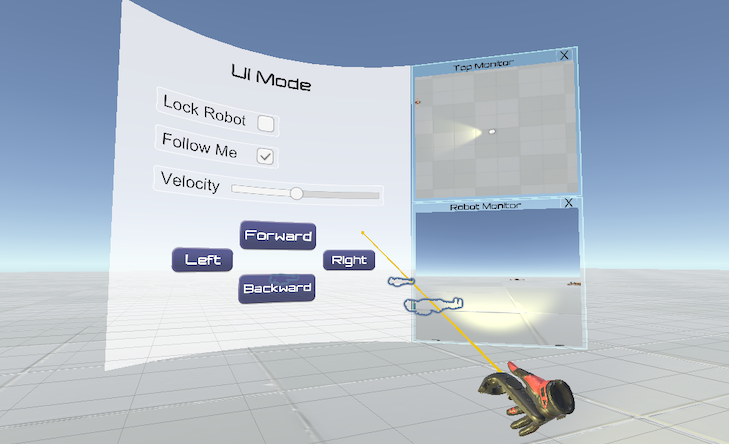
\includegraphics[height=5cm]{graphics/ui2.png}
    }
    \subfigure[Follow Function]{ 
        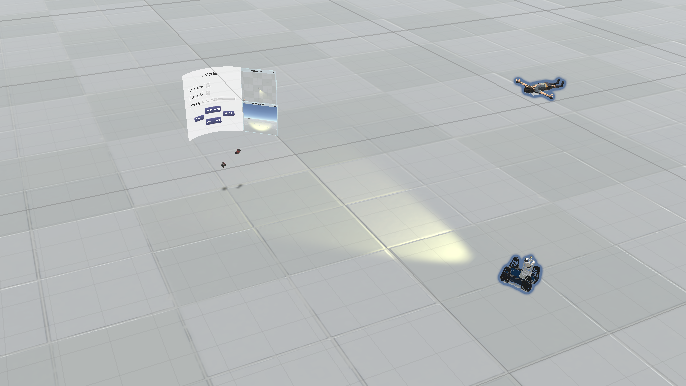
\includegraphics[height=5cm]{graphics/ui3.png}
    }
    \caption{UI Mode}
    \label{fig:ui} 
\end{figure}


\section{Test Scene}
In order to simulate the use of rescue robots in disaster scenarios, the test scenes were built to mimic the post-disaster urban environment as much as possible. The POLYGON Apocalypse \footnote{https://assetstore.unity.com/packages/3d/environments/urban/polygon-apocalypse-low-poly-3d-art-by-synty-154193}, available on the \gls{unity} Asset Store, is a low poly asset pack with a large number of models of buildings, streets, vehicles, etc. This resource pack was used as a base. Additional collision bodies of the appropriate size were manually added to each building and obstacle after the resource pack was imported, which was needed to help track the robot's driving crash in subsequent tests.

Considering that four operation modes need to be tested, four scenes with similar complexity and composition but different road layouts and placement of buildings were constructed. The similarity in complexity of the scenes ensures that the difficulty of the four tests is basically identical. The different scene setups ensure that the scene information learned by the user after one test will not make him understand the next test scene and thus affect the accuracy of the test data. 

The entire scene is initially invisible, and the visibility of each object in the test scene is gradually updated as the robot drives along. Ten interactable victim characters were placed in each test scene. The placement can be next to the car, the house side and some other reasonable places.

\begin{figure}[htbp]
    \centering
    \subfigure[Obstacle]{
        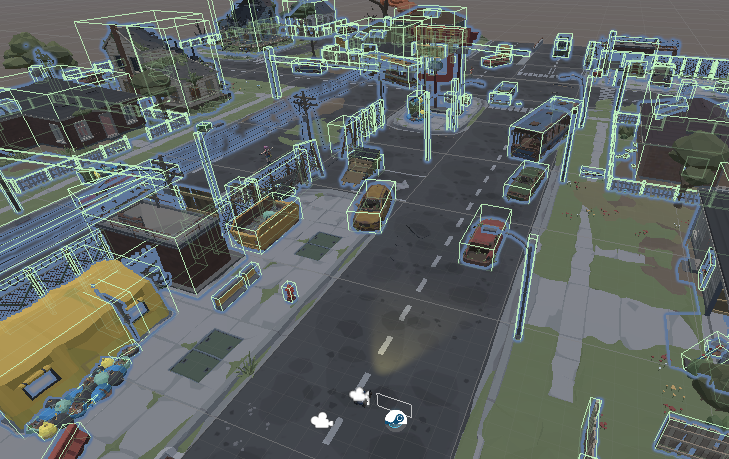
\includegraphics[height=5cm]{graphics/testCollider2.png}
    }
    \subfigure[Victims]{
        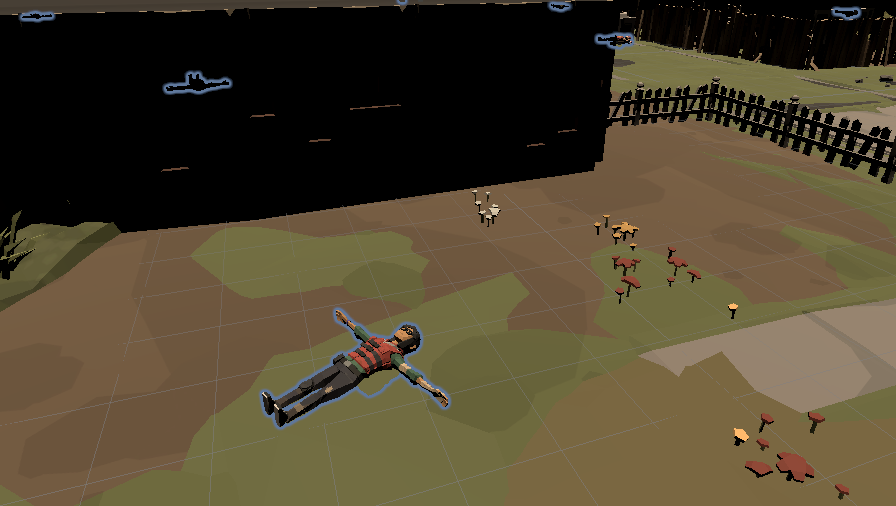
\includegraphics[height=5cm]{graphics/testVictim4.png}
    }
    \caption{Test Scene}
    \label{fig:testscene} 
\end{figure}